% !TEX TS-program = pdflatex
% !TeX spellcheck = en_US
% !TEX root = main.tex

\begin{figure}[t]
  \centering
  \subfloat[Sample GUI form\label{form1}]{
      \centering
      
\includegraphics[scale=0.35]{form1.png}
  }
  \vskip5mm
  \subfloat[Sample GUI form structure\label{form1-structure}]{
  \scalebox{0.5}{
  \begin{tikzpicture}
    \node[rectangle,draw] (check) at (12, 2.5) {
\includegraphics[scale=0.7]{check.png}};
    \node[rectangle,draw] (label) at (8.7, 0)  {
\includegraphics[scale=0.7]{label.png}};
    \node[rectangle,draw] (combo) at (15.3, 0) {
\includegraphics[scale=0.7]{combo.png}};
    \begin{scope}
      \node[rectangle,dashed,draw,fit=(label)(combo),minimum height=2cm,minimum width=12cm] (composite) (0, 0) {};
    \end{scope}
    \path[draw,->] (label.east) -- node[above] {\emph{descr}} (combo.west);
    \path[draw,->] (check.south) -- node[right] {\emph{order}} (12,1);
  \end{tikzpicture}}}
\vskip5mm
\subfloat[Sample GUI form layout\label{form1-layout}]{
  \scalebox{0.5}{
  \begin{tikzpicture}
    \node (label) at (7.3, 2.65) {\emph{justify}};
    \node[rectangle,draw] (check) at (9.45, 1.8) {
\includegraphics[scale=0.7]{check.png}};
    \node[rectangle,draw] (label) at (8.91, 0  ) {
\includegraphics[scale=0.7]{label.png}};
    \node[rectangle,draw] (combo) at (15.5, 0  ) {
\includegraphics[scale=0.7]{combo.png}};
    \begin{scope}
      \node[rectangle,dashed,draw,fit=(label)(combo)] (composite) (0, 0) {};
    \end{scope}
    \path[draw,<->] (label.east) -- node[above] {\emph{inset}} (combo.west);
    \path[draw,<->] (check.south) -- node[right] {\emph{inset}} (9.47,0.7);
    \path[draw,-] (6.7,3) -- (6.7,-0.4);
  \end{tikzpicture}}}
\vskip5mm
\subfloat[Sample GUI guideline rule\label{gdrule}]{
  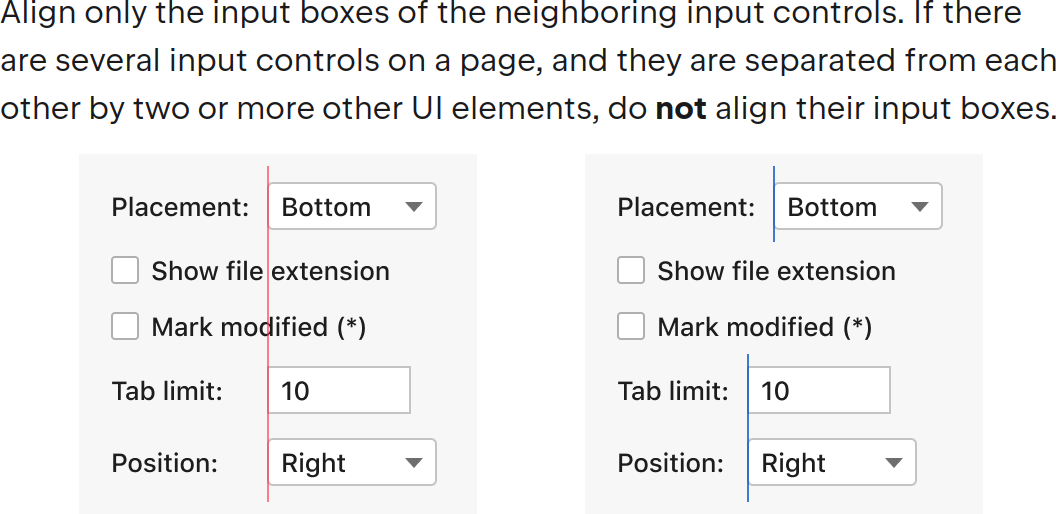
\includegraphics[scale=0.2]{jbg-10.png}
}

\caption{GUI form example, structure, layout, and guideline}
\label{form1-structure-layout}
\end{figure}



\begin{figure*}[t]
\begin{verbnobox}[\fontsize{10pt}{10pt}\selectfont]
ordered main_group (
  Label "Type" describes TextEdit "Any" { width=200 }
  Label "Owner" describes TextEdit "Anyone" { width=200 }
  Label "Has the words" describes TextEdit "Enter words found in the file" {
   width = 400
  }
  Label "Item name" describes
    TextEdit "Enter a term that matches part of the file name" {
      width = 400
    }
  (Label "Location" describes
    (TextEdit "Anywhere" { width = 200 }) dominates
    ordered location_checkboxes (
      Label "In trash"  describes CheckBox in_trash_checkbox
      Label "Starred"   describes CheckBox starred_checkbox
      Label "Encrypted" describes CheckBox encrypted
    )
  )
  Label "Date modified" describes  TextEdit "Any time" { width=200 }
  Label "Approvals" describes
    ordered approvals_checkboxes (
      Label "Awaiting my approval" describes CheckBox awaiting_checkbox
      Label "Requested by me" describes CheckBox requestred_checkbox
  )
  Label "Shared to" describes
    TextEdit "Enter a name or email address..." { width=400 }
  Label "Follow-ups" describes TextEdit "---" { width=200, height=35 }
)
Button "Search" approves^ main_group
Button "Reset" cancels^ main_group
\end{verbnobox}
\caption{Google Drive Search Settings Dialog Structure Description}
\label{gd_structure}
\end{figure*}

\begin{figure*}[t]
    \begin{subfigure}[t]{.45\textwidth}
        \vspace{-18em}
        \centering
        \begin{minipage}{6cm}
        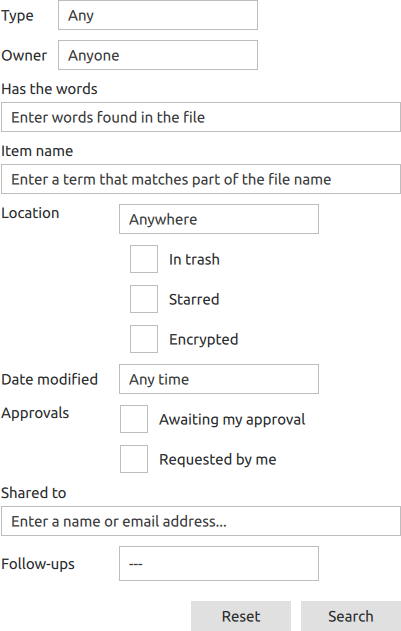
\includegraphics[scale=0.25]{google-drive-search-setting-output2.png}
        \end{minipage}
        \caption{If label describes controls which are ``too long'', then place them vertically}
    \end{subfigure}\hspace{1cm}
    \begin{subfigure}[t]{.45\textwidth}
      \centering
      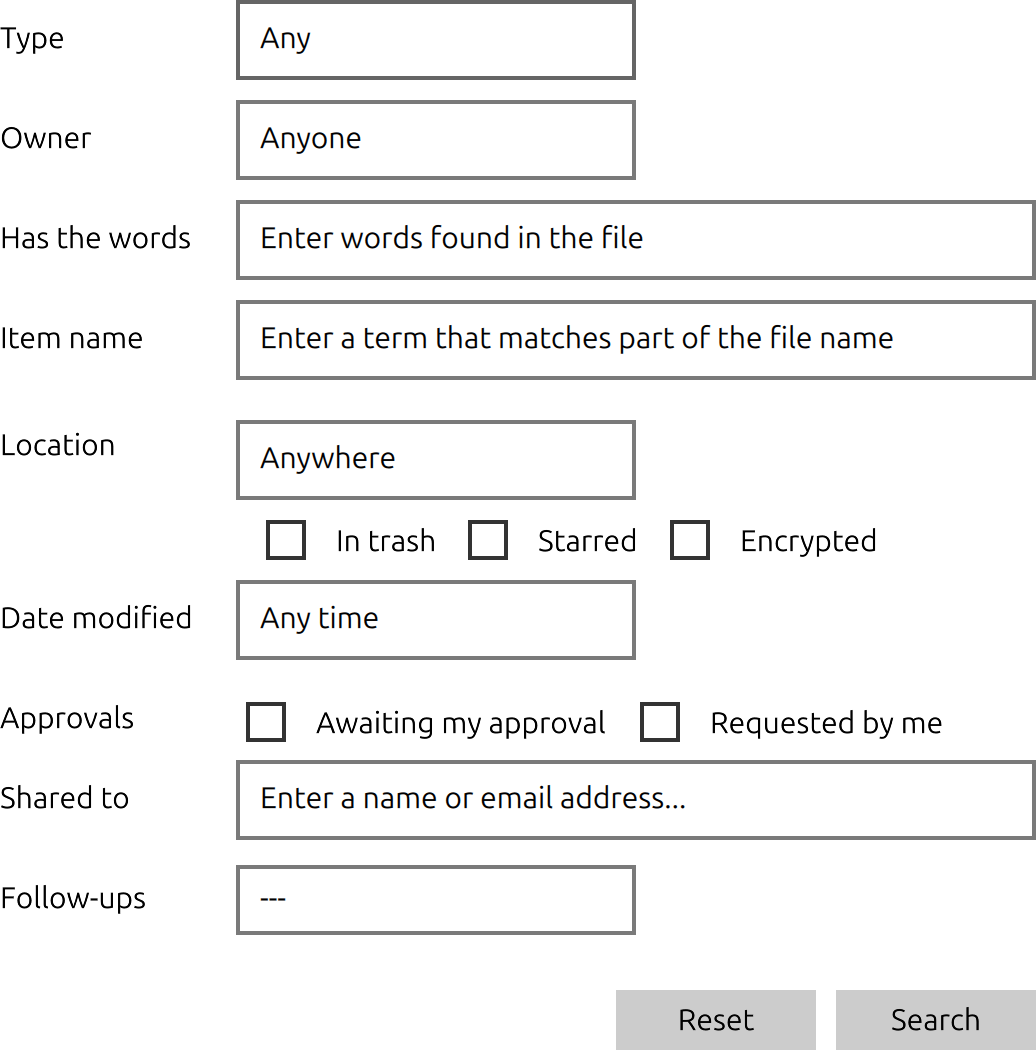
\includegraphics[scale=0.25]{google-drive-search-setting-output3.png}
      %\vskip17.5mm
      \caption{The same, but the constant for ``too long'' was decreased}
    \end{subfigure}
    \caption{Google Drive Search Settings Dialog Layouts}
    \label{fig:QMLtwoGuidelines}
\end{figure*}


\begin{figure*}
	\centering
    \begin{tabular}{m{85mm}m{6cm}}
      \begin{lstlisting}[basicstyle=\small]
ordered (
  Label "Short label"
    describes TextEdit "Text 1"
  Label "Loooooong label"
    describes TextEdit "Text 2"
)
      \end{lstlisting} &
      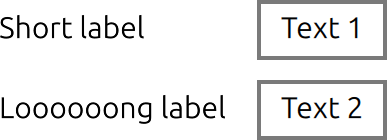
\includegraphics[scale=0.4]{Example1-Qt-QML.png} \\
      \hline
      \begin{lstlisting}[basicstyle=\small]
ordered (
  Label "Looooong label"
    describes TextEdit "Text 1"
  Label "Medium label"
    describes TextEdit "Text 2"
  Label "Short"
    describes TextEdit "Text 3"
  )
      \end{lstlisting} &
      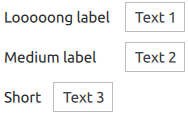
\includegraphics[scale=0.4]{Example2-Qt-QML.png} \\
      \hline
      \begin{lstlisting}[basicstyle=\small]
ordered (
  Label "Short label"
    describes TextEdit "Text 1"
  Label "Check box label"
    describes CheckBox _
  Label "Looooong label"
    describes TextEdit "Text 2"
)
      \end{lstlisting} &
      \vspace{1em}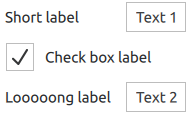
\includegraphics[scale=0.4]{Example4-Qt-QML.png} \\
      \hline
      \begin{lstlisting}[basicstyle=\small]
ordered (
  Label "L 1"     describes CheckBox _
  Label "Lab 2"   describes CheckBox _
  Label "Label 3" describes CheckBox _
  Label "Label 4" describes CheckBox _
  Label "L 5"     describes CheckBox _
  Label "Lab 6"   describes CheckBox _
)
      \end{lstlisting} &
      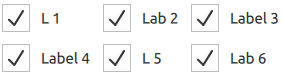
\includegraphics[scale=0.4]{Example5-Qt-QML.png} \\
    \end{tabular}
    \caption{Examples of structures (left) and synthesized layouts (right)\\
      w.r.t. JetBrains guidelines}
    \label{fig:evaluation}
  \end{figure*}
